\chapter{Stand der Technik}
\label{ch:StandDerTechnik}

Das erste \gls{rfid}-System wurde von den Allierten im Zweiten Weltkrieg eingesetzt. Deren Freund-Feind-Erkennung funktionierte über eine passive Reflektion der Radarwellen, welche auf die Frequenz der Radarsender geeicht war. Verbündete Flieger ergaben dadurch ein viel stärkeres Signal und waren als hellere Punkte erkennbar (\cite{chawla2007}, \cite{uswardep1946_3}). In den 1960er wurden in den USA verschiedenste Patente angemeldet, welche sich das Prinzip der elektromagnetischen Induktion zunutze machen, um sich gegenüber einem Sender zu identifizieren. Die Adaption der Technologie liess jedoch auf sich warten, \citeauthor{want2004} identifiziert als Grund dafür die fehlende Marktviabilität, die Ausgereiftheit der Technologie selbst und die Adaptionskosten \parencite{want2004}. All dies hat sich in den 60 Jahren seither geändert und \gls{rfid} ist eine etablierte Technologie, welche in verschiedensten Sparten eingesetzt wird.

\section{Technologische Grundlagen}

% Funktionsweise Transponder / Interrogator

% Active/Passive

Bei der Funktionsweise von \gls{rfid} Tags muss man zwischen zwei Funktionalitäten unterscheiden, welche auf die Entfernung zwischen Transponder und Interrogator abhängig sind. Im Nahbereich (engl. Near-Field \gls{rfid}) funktioniert die Stromversorgung über magnetische Induktion (die Arbeitsspannung der Chips liegt im Mikro- bis Miliwattbereich). Die Kommunikation zwischen Interrogator und Transponder wird über "load modulation"\ realisiert. Dies bedeutet, dass der Transponder, aktiviert durch das Feld des Interrogator, selber beginnt ein Feld auszustrahlen. Dadurch entstehen Interferenzen im Feld welche sich durch minimale Spannungsänderungen in der Spule des Interrogators messen lassen \parencite{want2006}. Die Distanz des Nahfelds ist durch die Gleichung \ref{NearFieldEM} gegeben. Für \gls{HF} Tags (wie diejenigen die auch in der Speicherbibliothek verwendet werden) ist die Betriebsfrequenz durch den ISO Standard 18000-3 auf 13.56MHz festgelegt und ergibt damit eine Distanz von 3.519m für das Nahfeld.

\indexequation{d=\frac{\lambda}{2\pi}}{Reichweite des reaktiven Nahfelds}{NearFieldDistance}
\indexequation{\lambda=\frac{c}{f}}{Definition der Wellenlänge $\lambda$ in Abhängigkeit der Lichtgeschwindigkeit c}{Wavelength}
\indexequation{d=\frac{c}{2\lambda\pi}}{Definition der Wellenlänge in Gleichung \ref{NearFieldDistance} eingesetzt}{NearFieldEM}

Im Fernfeldbereich erhält der \gls{rfid} Tag direkt über die ausgestrahlte Elektromagnetischen Wellen. Die Abnahme der Energiedichte auf Distanz ist dabei proportional zu $\frac{1}{r^2}$. Dennoch ist es durch Fortschritte in der Miniaturisierung und besserer Energieeffizienz moderner Halbleiter und Chips möglich dadurch \gls{UHF} Tags mit Strom zu versorgen. Die Kommunikation funktioniert mittels "back scattering"\ - eine Antenne welche auf eine bestimmte Frequenz eingestellt ist, absorbiert den Grossteil der Wellen die gesendet werden. Passt jedoch die Impedanz nicht genau, so reflektiert die Antenne ein Teil des Signals an die Quelle, den Interrogator, zurück. Durch das Anpassen der Impedanz der Antenne über die Zeit, kann mehr oder weniger des Signals reflektiert und so eine Nachricht codiert werden \parencite{want2006}.

\begin{figure}[htb]
	\centering
	\begin{subfigure}[b]{0.8\linewidth}
		\centering
		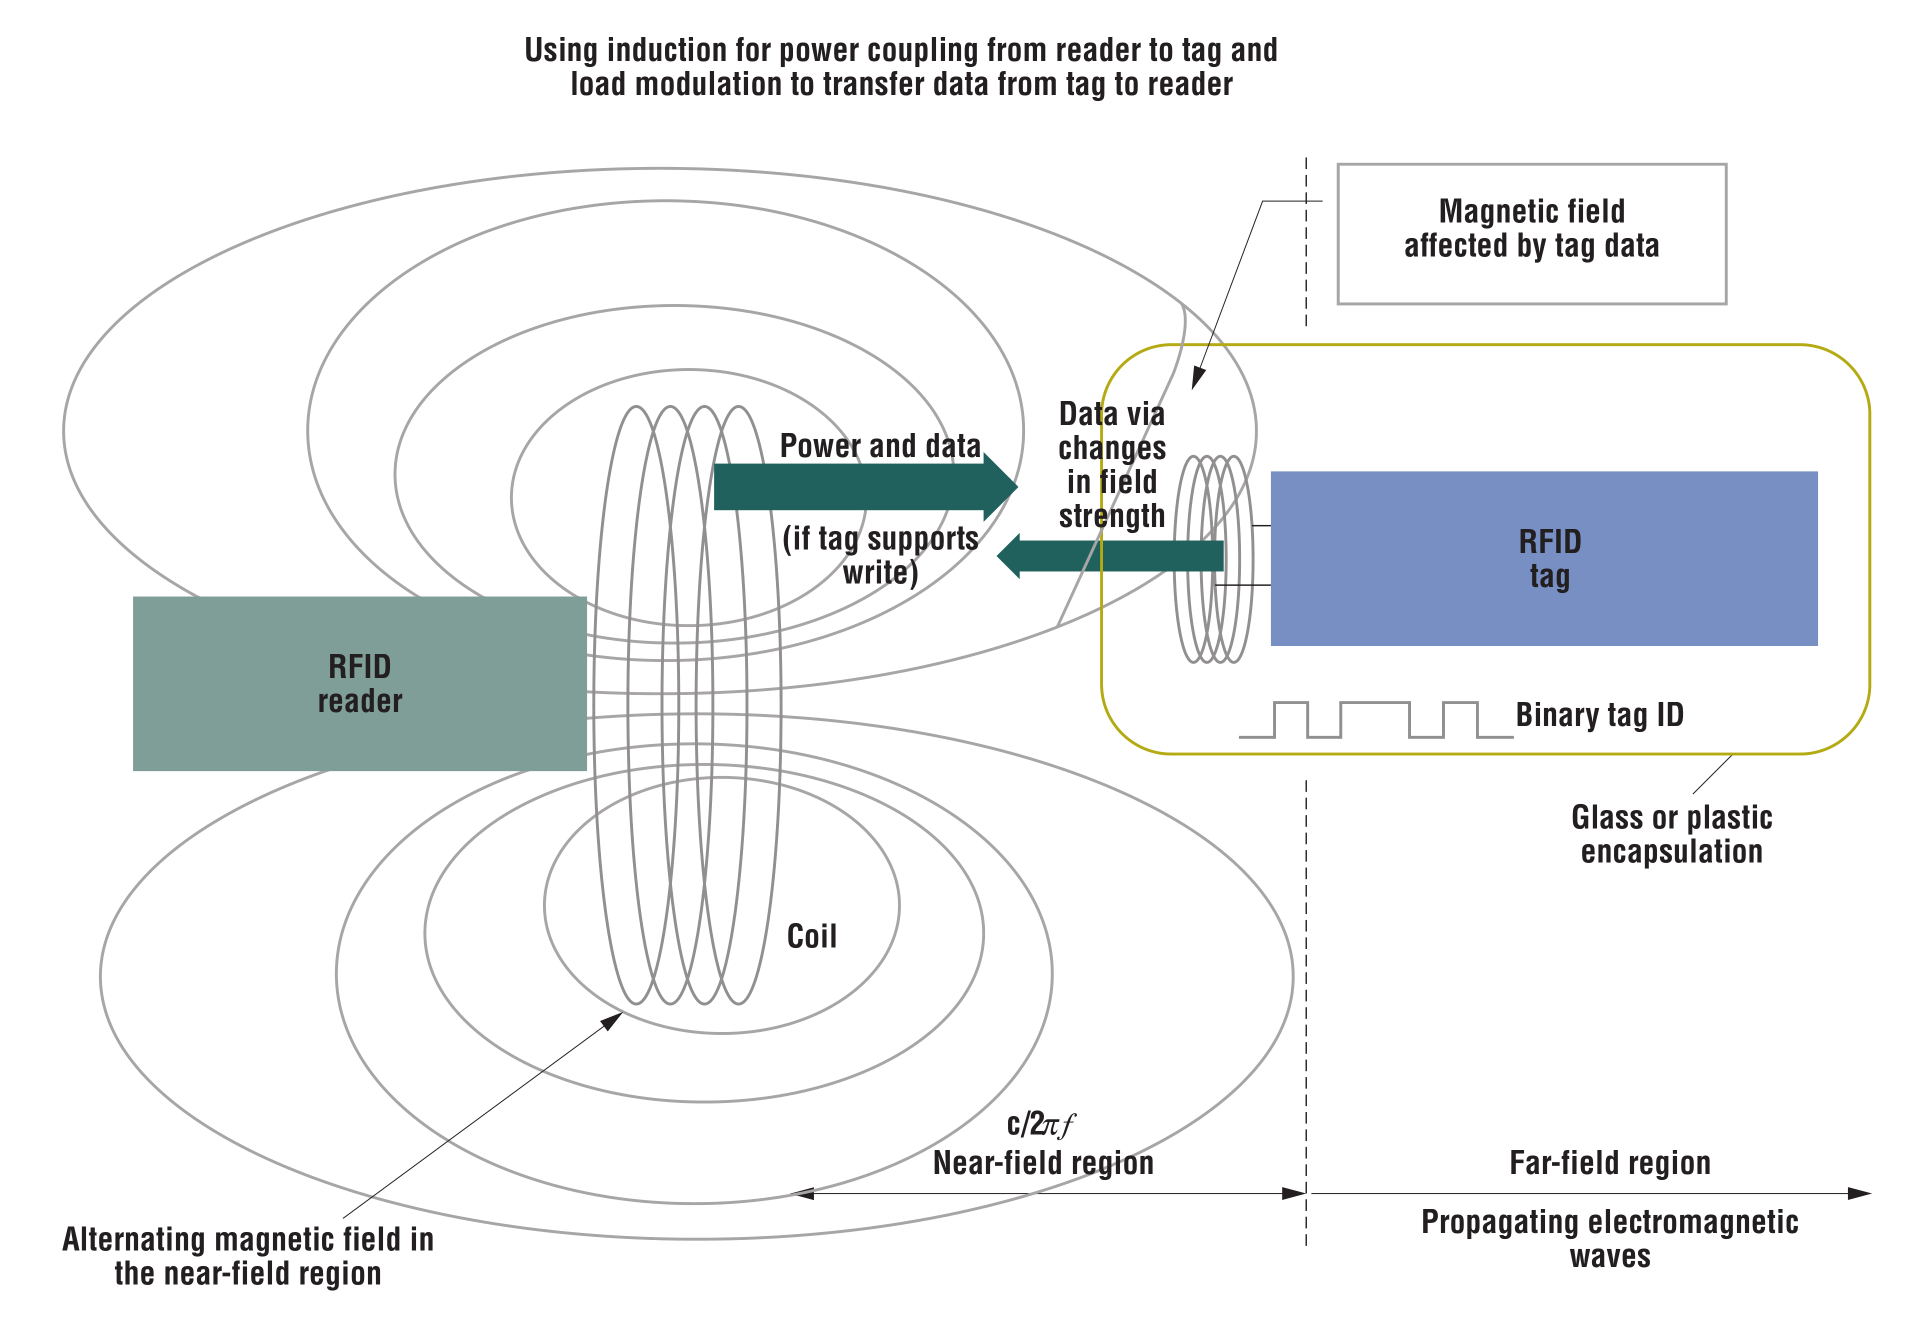
\includegraphics[keepaspectratio,width=\linewidth]{InductionCoupling}
		\caption{Magnetische Induktion und "load modulation"}
	\end{subfigure}
	\begin{subfigure}[b]{0.8\linewidth}
		\centering
		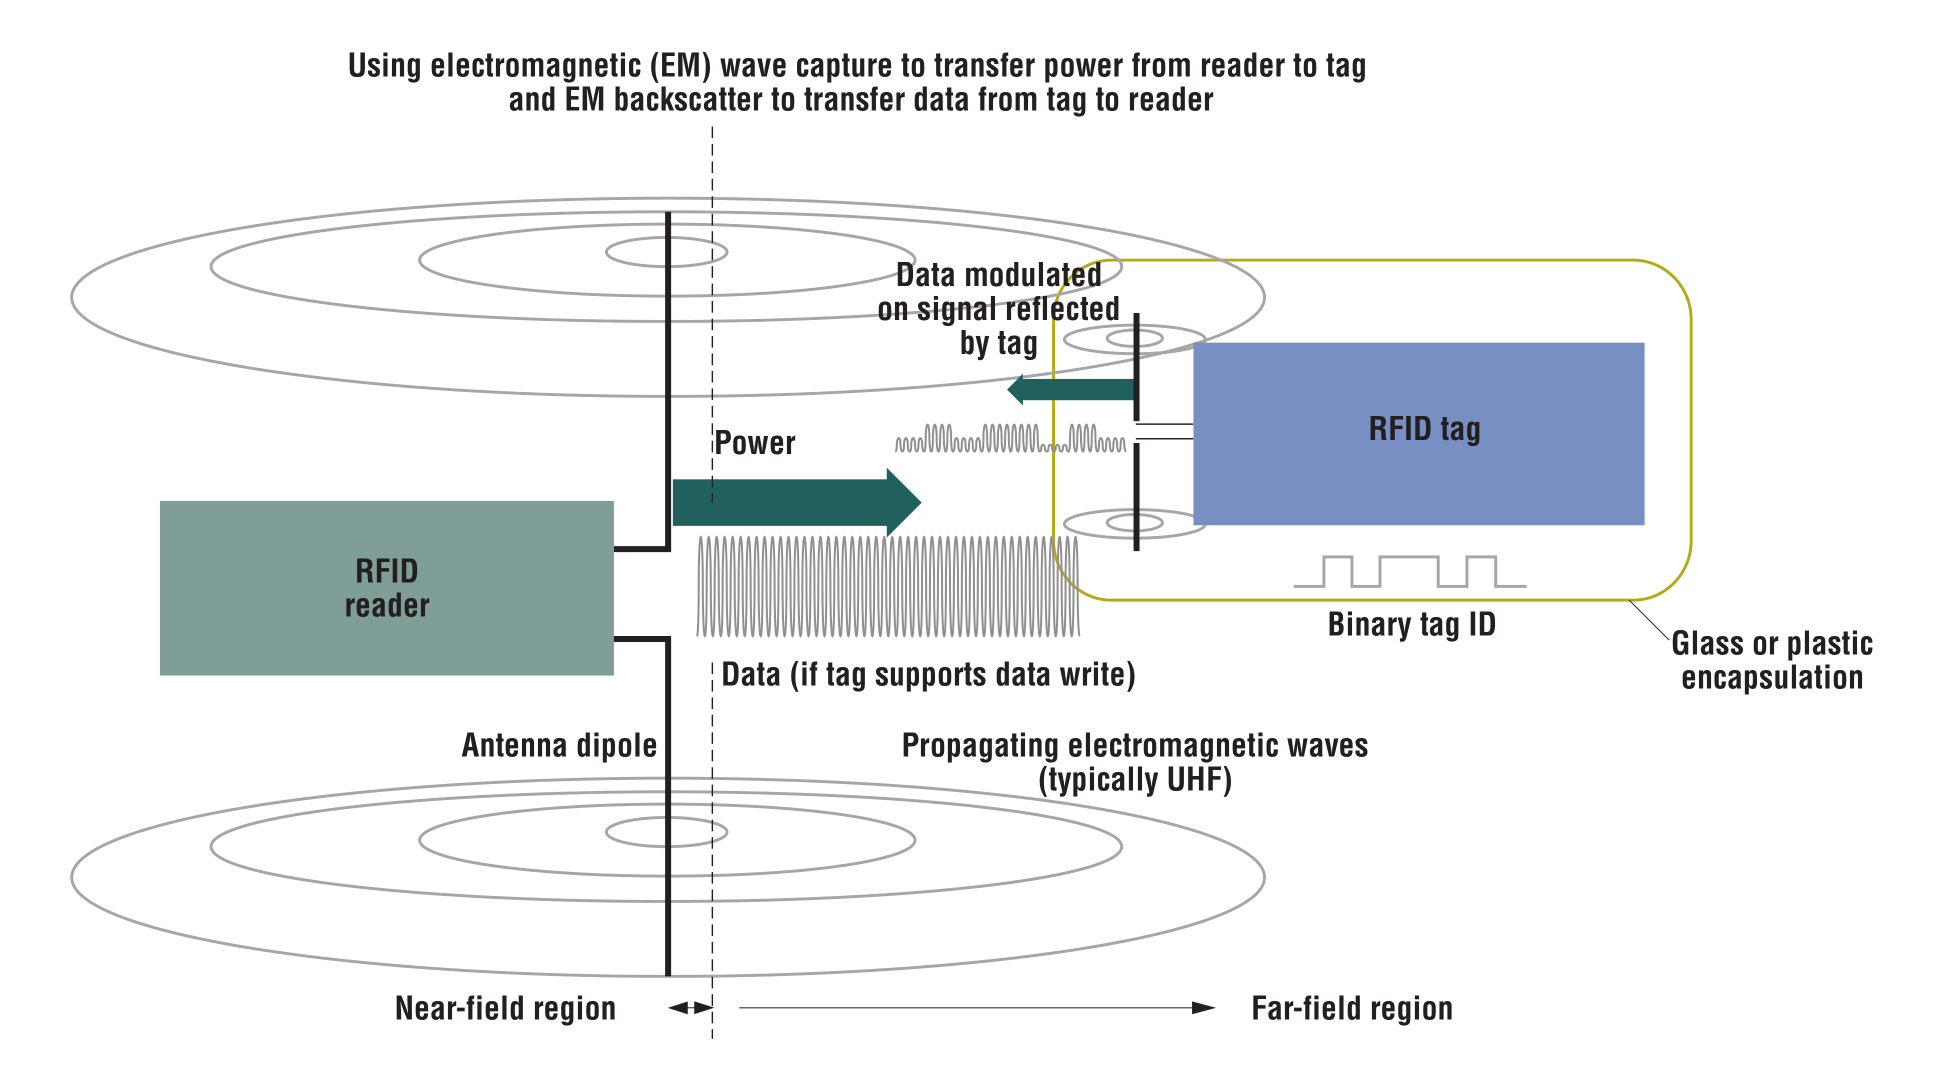
\includegraphics[keepaspectratio,width=\linewidth]{Backscattering}
		\caption{EM Wellentransmission und "backscattering"}
	\end{subfigure}
	\caption{Funktionsweisen von Nah- und Fernfeld \gls{rfid} Tags graphisch dargestellt \parencite{want2006}}
\end{figure}

\section{Technische Konzepte}

% CSMA Strategies

% Charakteristiken der unterschiedlichen Frequenzen

\section{Anwendungen}

% NFC, Regulatorische Vorschriften v.a. im Bezug zur Schweiz